The metrics usable for the tasks described in Section~\ref{sec:introduction} are manifold.
As not all metrics are suitable for all the work done by the model.
We therefore split this section into two subsections.

\subsection{Compression}\label{subsec:compression}
For compression, the most straightforward metric is to measure the reduction of memory required to
store the data.
To normalize over image resolution, we choose to evaluate the \ac{bpp}.

The second, and less objective measure, is image similarity after reconstruction.
While the \ac{mse} and by transfer \ac{psnr} describe pixel-wise similarity very well, it is not
always optimal to judge perceived similarity for humans, as can be seen in Figure~\ref{fig:mse_ssim}.

\[
\text{MSE} = \frac{1}{n} \sum_{i=1}^{n} (y_i - x_i)^2 \quad \quad \text{PSNR} = 10 \cdot \log_{10} \left( \frac{\text{MAX$^2$}}{\text{MSE}} \right)
\]
where $\text{MAX}$ is the maximum possible pixel value (255 for our 8-bit images).

\begin{figure}[ht]
    \centering
    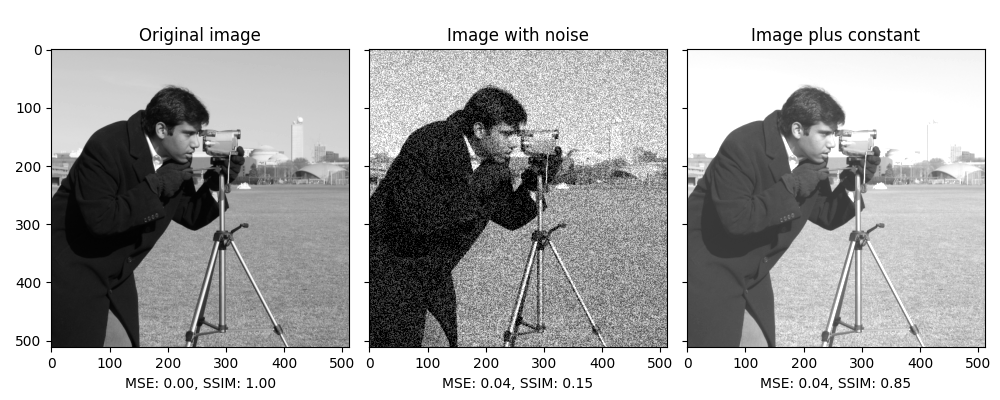
\includegraphics[width=0.6\textwidth]{images/ssim_mse}
    \caption{Two images with the same \ac{mse} with reference from~\cite{scikit-ssim}}
    \label{fig:mse_ssim}
\end{figure}

To overcome these limitations we use the \ac{ssim}, a metric working under the assumption that human visual
perception is highly adapted for extracting structural information from a scene~\cite{ssim}.

\[
\text{SSIM}(x, y) = \frac{(2\mu_x \mu_y + C_1)(2\sigma_{xy} + C_2)}{(\mu_x^2 + \mu_y^2 + C_1)(\sigma_x^2 + \sigma_y^2 + C_2)}
\]
$\text{where } C_1 = (K_1L)^2 \text{ and } C_2 = (K_2L)^2 \text{ are constants to avoid dividing by zero.}$


Even though this analysis favours \ac{ssim}, we use \ac{mse} as our loss function for our baseline models,
since the \ac{vq} implementation we plan to replicate does the same, and we want to maximize comparability.
We use \ac{ssim} for result evaluation, and add \ac{psnr} values for further experiments.

\subsection{Image Generation}\label{subsec:image-generation}
An important metric in Image Generation is the \ac{nll} normalized to the amount of pixels (dimensions) in an image, given in bits/dim.
It is used to argue about the strong performance of the \ac{vq} in the paper.
A lower number indicates a higher likelihood of generating the test data given our model.
The bits/dim number is rooted in information theory, and describes the average number of bits required to
compress the test data with the entropy coding scheme that is optimal for a model~\cite{shannon}.

The \ac{fid}, introduced by~\cite{fid}, is another interesting metric.
It compares the distribution of features of a generator with that of real images via a network trained on a big
dataset, often also imagenet.

Another criterion not to be left out is the classic human turing test, as in evaluating the images by hand.
Even though this is not scalable, it is the ultimate classifier for human perception, and can be a good starting
point.

For metrics we decided not to use: The paper introducing \ac{fid} shows it is more consistent than the earlier and
similar inception score, so we excluded the latter.
Research advises against using Parzen Window Estimates~\cite{note_on_eval}, so we avoided them as well.

Since we have not yet implemented any image generation functionality, the value of these metrics remains to be evaluated.

TODO: INTRODUCE FORMULAS FOR THE CRITERIONS
